%! Author = Yilin
%! Date = 2025/1/27

To identify the effectiveness of national cybersecurity policies,
it is essential to analyze the correlation between the implementation of these policies and the subsequent trends in cybercrime.
By examining the distribution of cybercrimes and comparing it with the timing and content of various national policies,
we can discern patterns that highlight which measures are particularly effective or ineffective.
This analysis will focus on key metrics such as the reduction in
cybercrime incidents, the success rate of prosecutions, and the overall resilience of national cybersecurity infrastructures.
Through this data-driven approach,
we aim to provide actionable insights for the development and refinement of cybersecurity policies.
\subsection{Selection of Representative Centroid Countries}\label{subsec:selection-of-representative centroid-countries} %4.1
    Having constructed a clustering model to categorize countries into five clusters (T1 to T5) based on GCI and other relevant metrics,
    we now proceed to analyze the effectiveness of cybersecurity policies within each cluster.
    To ensure a representative and data-driven analysis,
    we will select one central country from each cluster that meets the following criteria:
    \begin{itemize}
        \item \textbf{Representativeness:}
        The selected country should typify the overall characteristics of its cluster,
        reflecting the general trends and patterns observed within that group.
        \item \textbf{Data Availability:}
        The country must have sufficient historical data on cybersecurity policies and legislation enacted over the past two decades,
        allowing for a comprehensive analysis of policy impacts.
    \end{itemize}
    By focusing on these representative countries,
    we aim to draw meaningful insights into the effectiveness of various cybersecurity policies and laws,
    which can then be generalized to other countries within the same cluster.
    
    \subsubsection*{Implementation Steps} %4.1.1
        To identify the representative country for each cluster,
        we first calculate the average GCI for each cluster.
        The average GCI, denoted as \(\overline{GCI}\), is computed as follows:
        \begin{equation}
            \overline{GCI} = \frac{\sum_{i=1}^{n} GCI_i}{n}\label{eq:4-1-1-1}
        \end{equation}
        where \(n\) is the number of countries in the cluster.
        Next, we compute the absolute deviation of each country's GCI from the cluster average:
        \begin{equation}
            \{ a|a= |GCI_i - \overline{GCI}| \}\label{eq:4-1-1-2}
        \end{equation}
        where \(a\) is the approach to the average \( \overline{GCI} \).
        The country with the smallest deviation is considered the most representative of its cluster.
        After this initial selection, we further filter out countries with insufficient or incomplete legal and policy documentation.
    
        Through this process, we identify the following representative countries for each cluster with their references:
        \bigskip
        \begin{table}
            \centering
            \caption{Representative Countries of Each Tie Based on GCI Division}
            \label{tab:representative-countries-of-each-tie-based-on-gci-division}
            \resizebox{0.6\linewidth}{!}{
                \begin{tabular}{ccccc}
                    \hline
                    \textbf{T1} & \textbf{T2} & \textbf{T3} & \textbf{T4}  & \textbf{T5} \\
                    \hline
                    United States & Japan & China & Costa Rica & Namibia \\
                    \hline
                \end{tabular}
            }
        \end{table}

    \subsubsection*{Visualizing Policy Impact Over Time} %4.1.2
        With the selected representative countries,
        we proceed to visualize the impact of cybersecurity policies on cybercrime trends.
        For each country, we plot a line graph where
        the x-axis represents time (from 2000 to 2023) and the y-axis represents the annual number of cybercrime incidents.
        To highlight the influence of policy implementations,
        we mark the data points corresponding to years in which cybersecurity policies or laws were enacted with an orange color.
        This visualization is presented in Figure~\ref{fig:representative-policy}.
    
        This allows us to preliminarily assess the effectiveness of the policies.
        Specifically:
        \begin{itemize}
            \item A downward trend in the line graph following the implementation of a policy (marked in orange)
            suggests that the policy may have been effective in reducing cybercrime.
            \item An upward or unchanged trend, on the other hand,
            may indicate that the policy was ineffective or had unintended consequences.
        \end{itemize}
    
        This initial analysis provides a broad overview of the impact of various policies and
        helps identify patterns that warrant further investigation.
        It also serves as a foundation for more detailed analysis of specific policies, guiding future research directions.
    
        \begin{figure}[htb]
            \centering
            \subfloat[US\cite{us}]{
                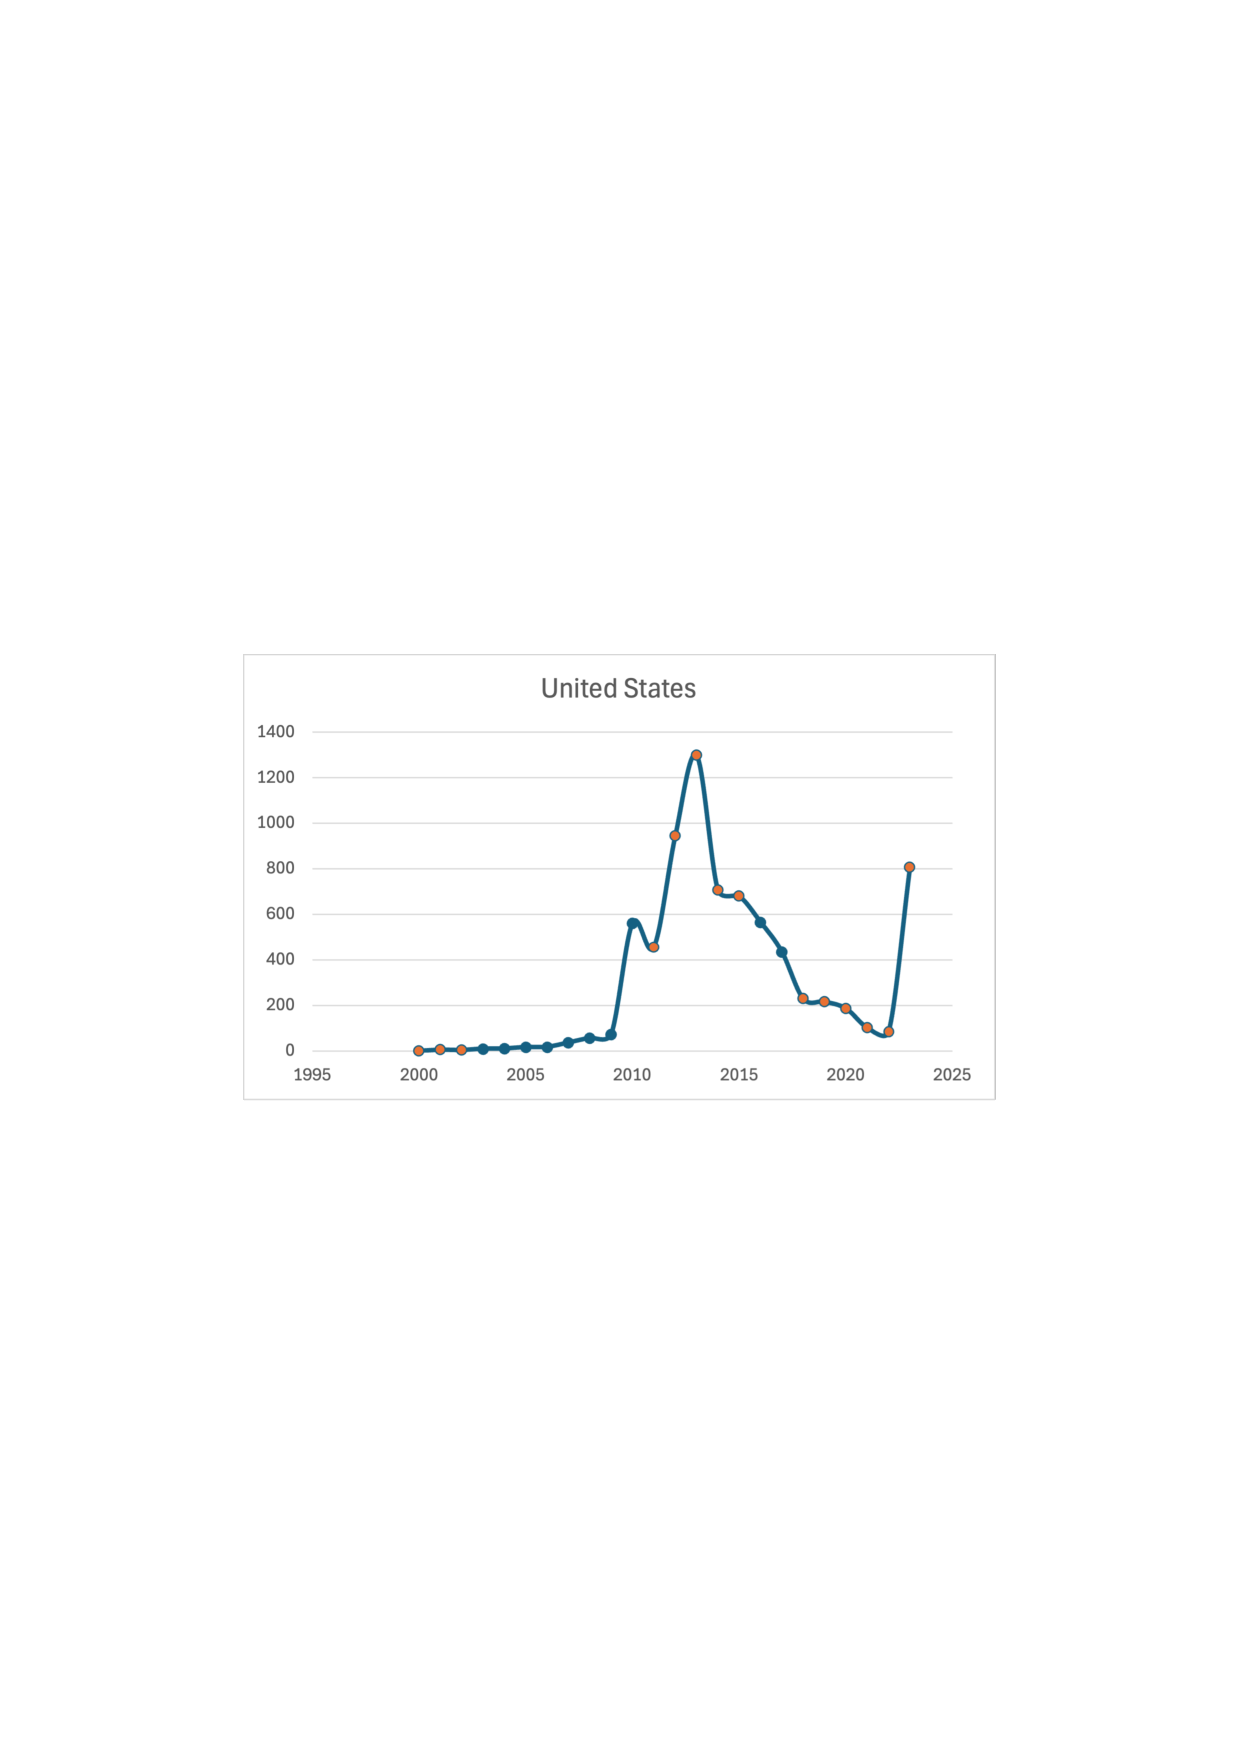
\includegraphics[width=0.45\linewidth]{../rsrc/policies/(T1)US_policy}
            }\hfill
            \subfloat[Japan\cite{jp}]{
                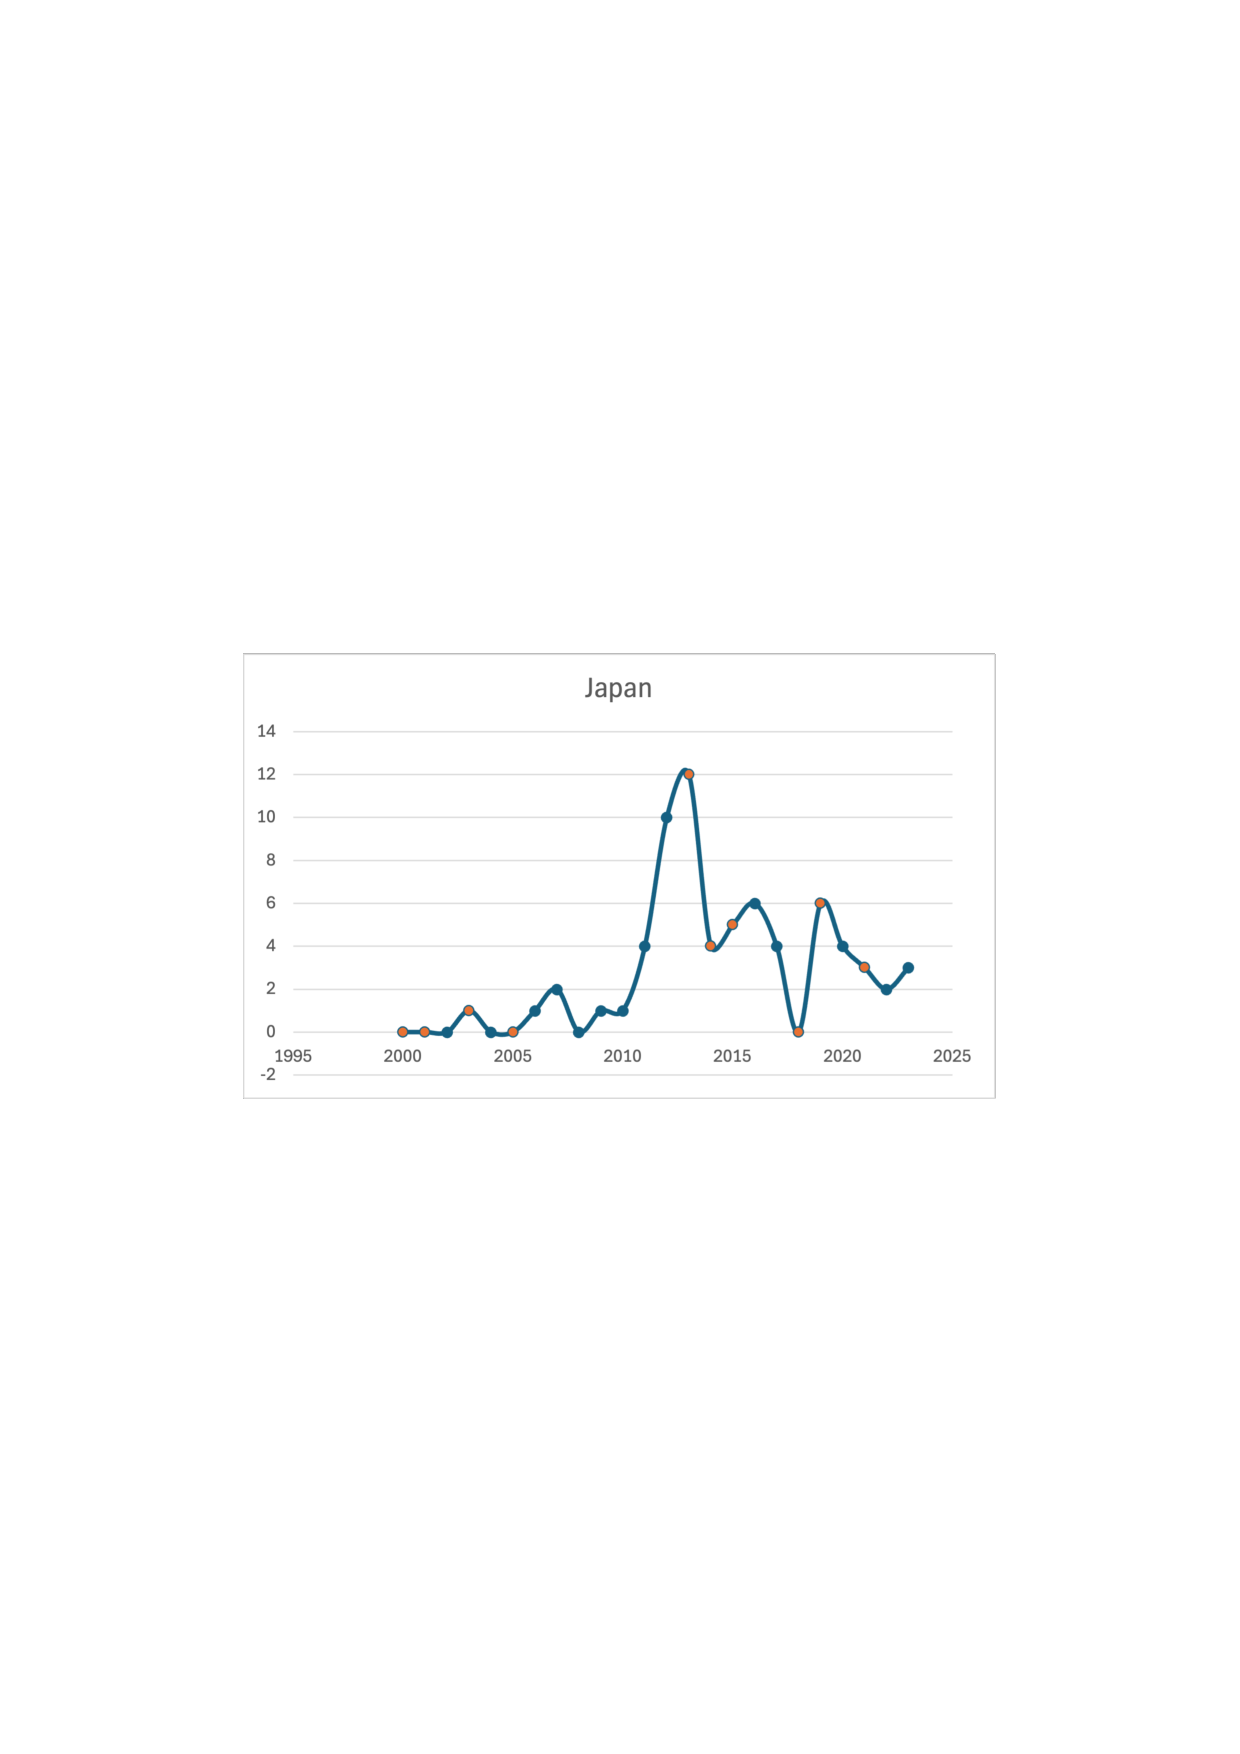
\includegraphics[width=0.45\linewidth]{../rsrc/policies/(T2)Japan_policy}
            }\\
            \subfloat[China\cite{ch}]{
                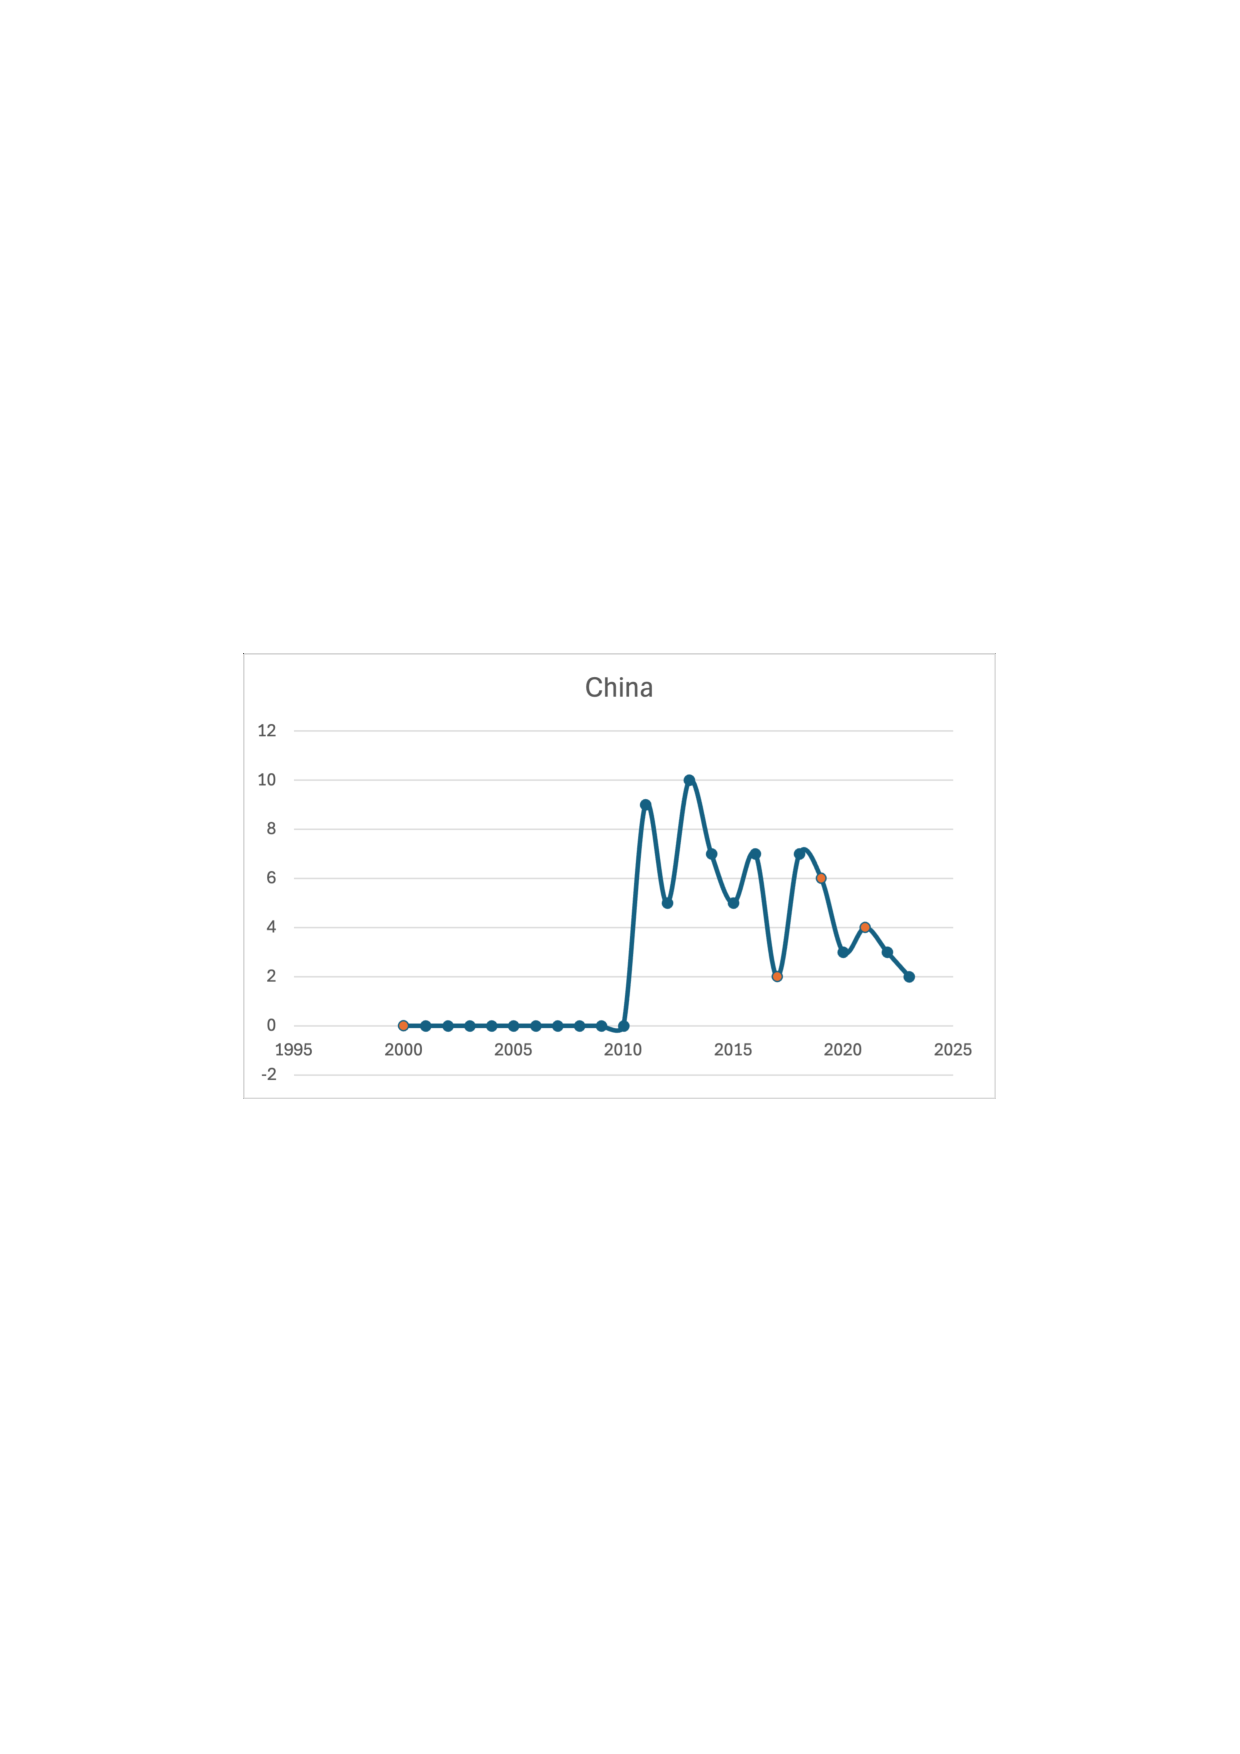
\includegraphics[width=0.3\linewidth]{../rsrc/policies/(T3)China_policy}
            }\hfill
            \subfloat[Costa Rica\cite{cr}]{
                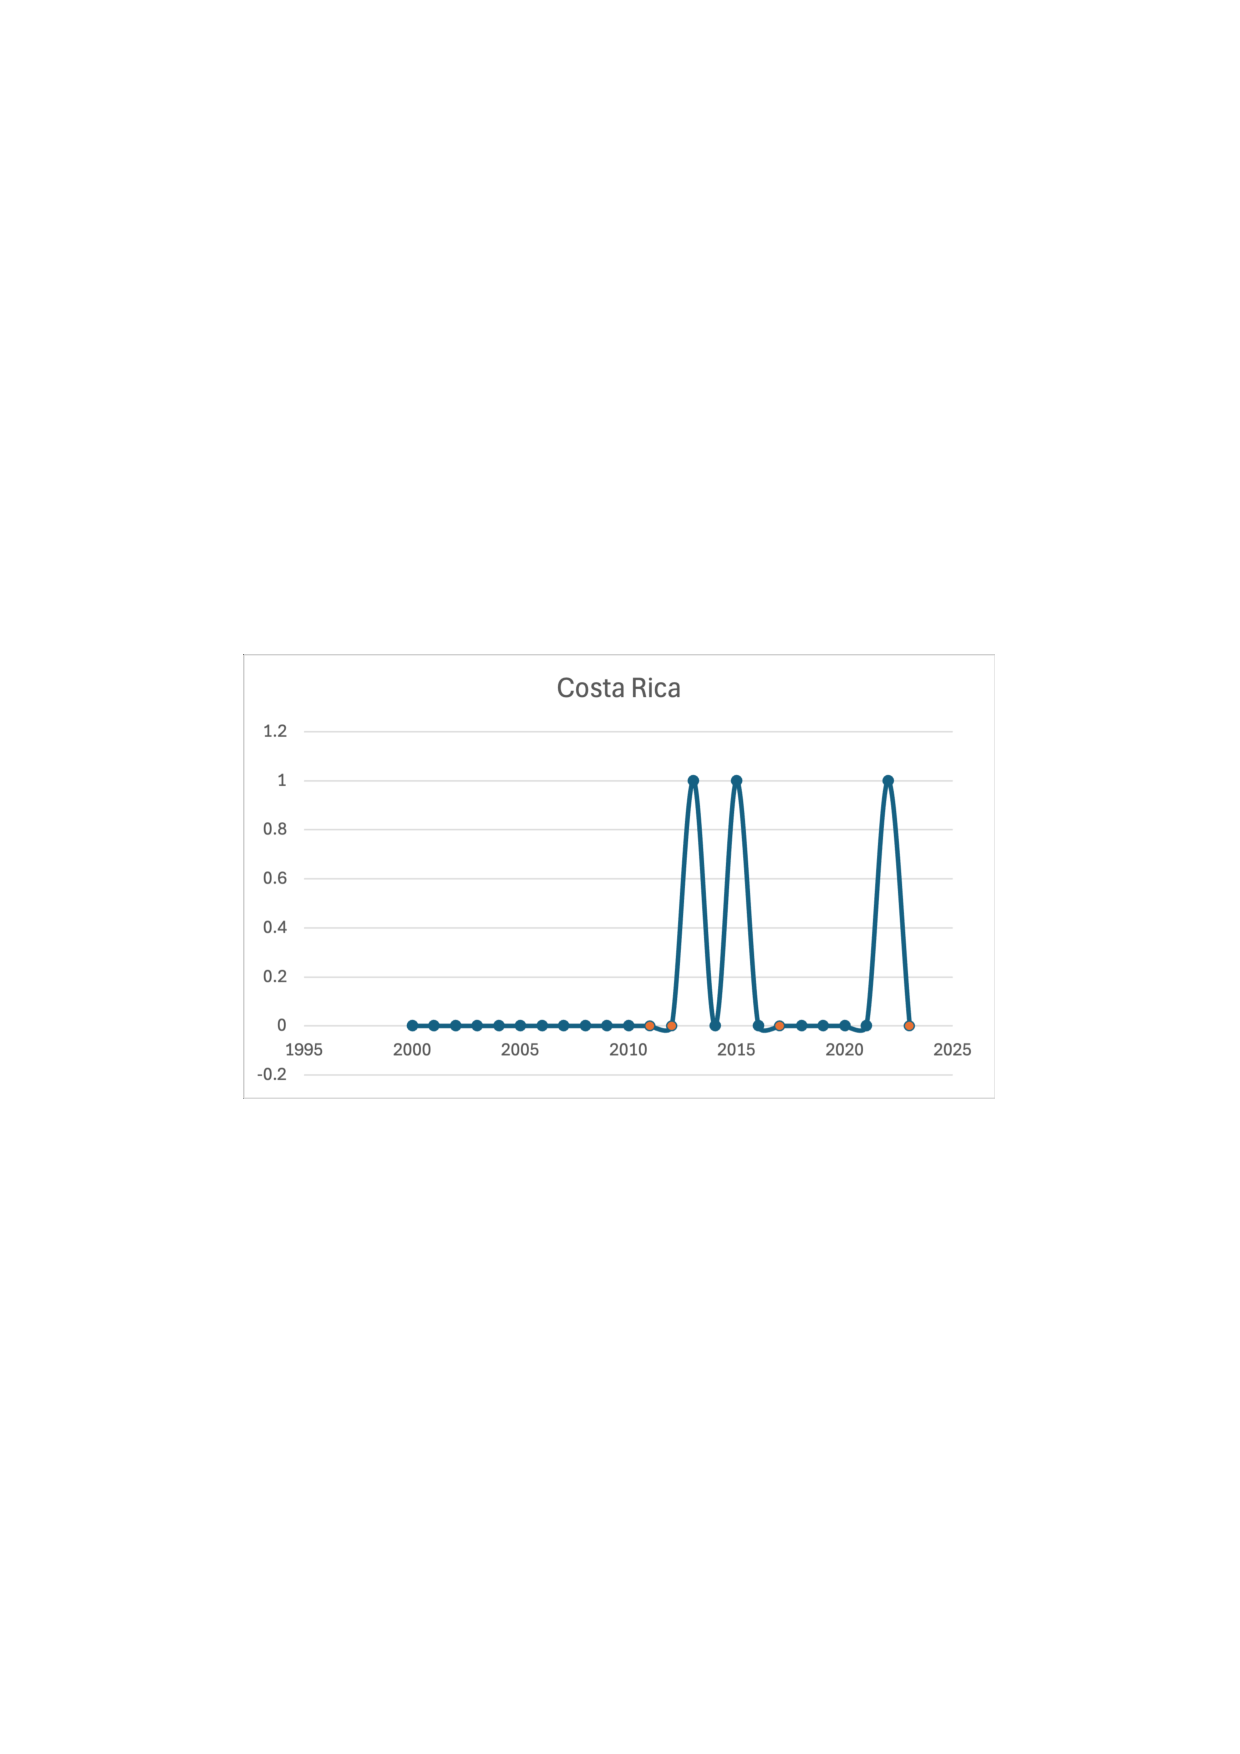
\includegraphics[width=0.3\linewidth]{../rsrc/policies/(T4)Costa_Rica_policy}
            }\hfill
            \subfloat[Namibia\cite{nb}]{
                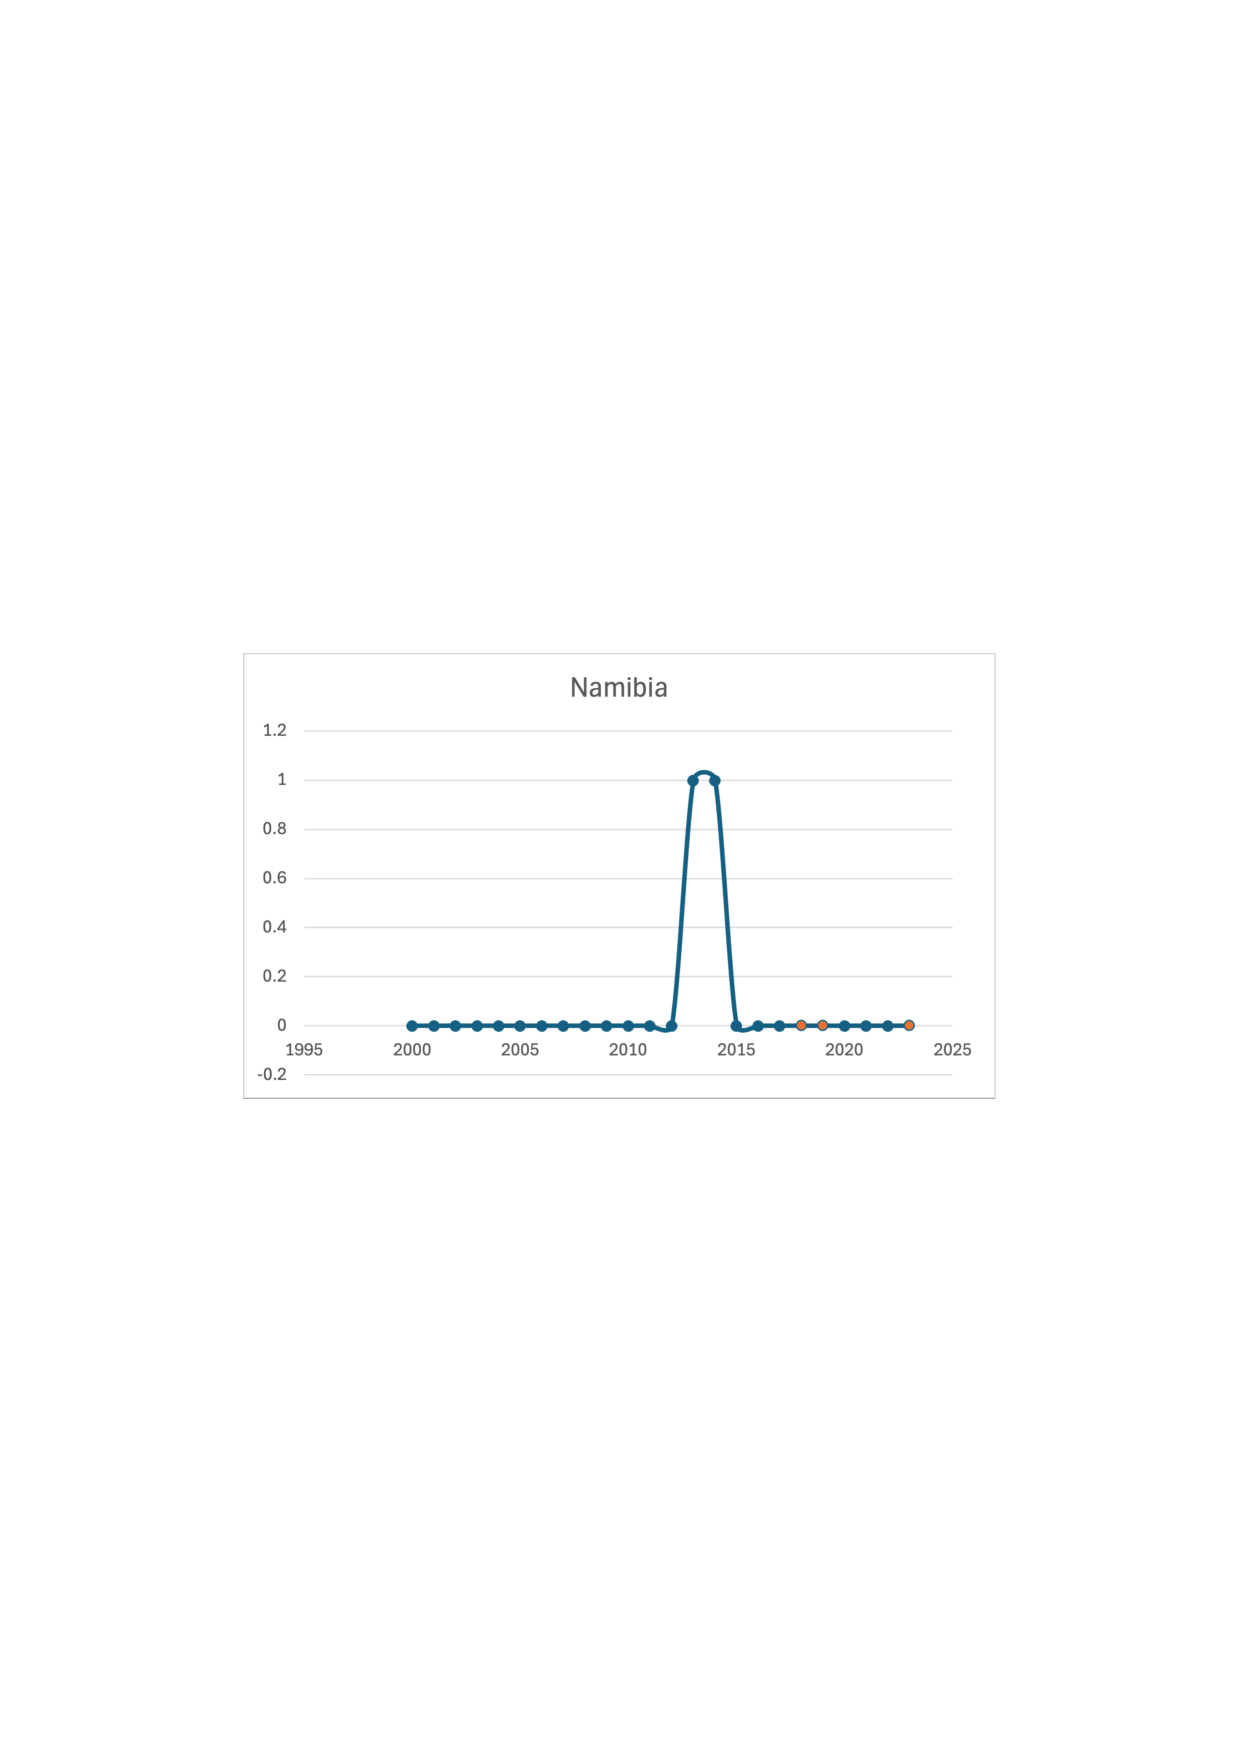
\includegraphics[width=0.3\linewidth]{../rsrc/policies/(T5)Namibia_policy}
            }\\
            \caption{National Tier Classification with Annual Legislation and Policy Releases}\label{fig:representative-policy}
        \end{figure}
    
\subsection{Categorizing Policies Based on Effectiveness}\label{subsec:categorizing-policies-based-on-effectiveness} %4.2
    From the line graphs, we categorize the enacted policies into three sets
    based on the average cybercrime metrics in the years following their implementation compared to the year of enactment.
    Drawing inspiration from fuzzy set theory,
    we assign a value of \(1\) to policies that are effective,
    \(-1\) to those with the opposite effect,
    and values between \(-1\) and \(1\) to policies with varying degrees of impact.
    Specifically:

    \begin{itemize}
        \item \textbf{Effective Policies:}
            These are policies where the average cybercrime metrics in the years following enactment
            are lower than those in the year of enactment.
            Examples include:
            \begin{itemize}
                \item National Institute of Standards and Technology (NIST) Cybersecurity Framework (2014)
                \item National Cyber Security Centre (NCSC) Establishment (2016)
                \item Investigatory Powers Act (2016)
                \item Cybersecurity Strategy (2013)
                \item Telecommunications Business Act Amendments (2019)
                \item Cryptography Law of the People’s Republic of China (2019)
            \end{itemize}

        \item \textbf{Counterproductive Policies:}
            These are policies where the average cybercrime metrics in the years following enactment
            are higher than those in the year of enactment.
            Examples include:
            \begin{itemize}
                \item Cyber Incident Reporting for Critical Infrastructure Act (CIRCIA) (2022)
                \item Quantum Computing Cybersecurity Preparedness Act (2022)
                \item Strengthening American Cybersecurity Act (2022)
                \item CHIPS and Science Act (2022)
                \item Cybersecurity Strategy (2018)
                \item Cybersecurity Law of the People’s Republic of China (2017)
            \end{itemize}

        \item \textbf{Neutral or Mixed-Impact Policies:}
            These are policies where
            the average cybercrime metrics show no significant change, or the impact is ambiguous.
    \end{itemize}

    This categorization provides a structured framework for analyzing the effectiveness of cybersecurity policies and
    serves as a basis for further investigation into the factors that contribute to their success or failure.
    
\subsection{Analysis of Effective Policies}\label{subsec:analysis-of-effective-policies} %4.3
    The effective policies, such as the
    \textbf{National Institute of Standards and Technology (NIST) Cybersecurity Framework (2014)},
    \textbf{National Cyber Security Centre (NCSC) Establishment 2016},
    \textbf{Investigatory Powers Act 2016}, and
    \textbf{Cryptography Law of the People’s Republic of China (2019)},
    share common characteristics in governance, international collaboration, technical regulation, and responsiveness to emerging threats.
    Through these mechanisms, they reduce opportunities for crime, increase the cost of cybercrime, and create a deterrent effect,
    ultimately leading to a significant decline in cybercrime incidents.

\subsection{Other cybercrime indicators}\label{subsec:other-cybercrime-indicators} %4.4
    For certain specific metrics of cybercrime, such as the proportion of successful crimes and the proportion of reported crimes,
    we focus on countries with more comprehensive data available in VCDB .
    Given the limited data coverage, we select countries with sufficient data for analysis,
    such as the United States, the United Kingdom, and Canada.
    These countries provide a robust dataset for examining trends in cybercrime success rates and reporting rates,
    allowing us to draw meaningful insights into the effectiveness of cybersecurity policies and practices in these regions.

    \subsubsection*{Impact on Cyberattack Success Rates} %4.4.1
        The line graphs depicting the crime success rate over time for the United States and Canada are shown in Figure
        ~\ref{fig:mitigated-attempts}.
        The figure illustrates that the establishment of the \testbf{National Cyber Security Centre (NCSC) Establishment 2016}
        has been particularly effective in reducing the success rate of cybercrimes.
        In contrast, other policies enacted during the same period do not appear to have had a significant impact
        on curbing the success rate of cybercrimes.
        This highlights the importance of centralized, technically-focused initiatives in mitigating the effectiveness of cyberattacks.
        \begin{figure}[htb]
            \centering
            \subfloat[US\cite{us}]{
                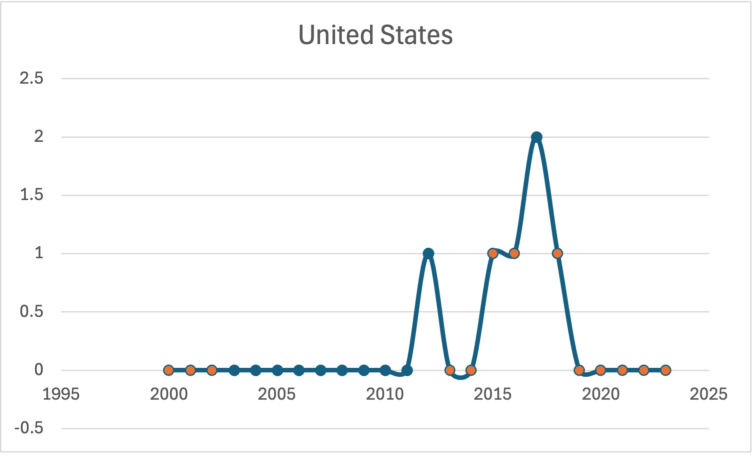
\includegraphics[width=0.45\linewidth]{../rsrc/other_policies/US_policy_nearMiss}
            }\hfill
            \subfloat[Canada\cite{ca}]{
                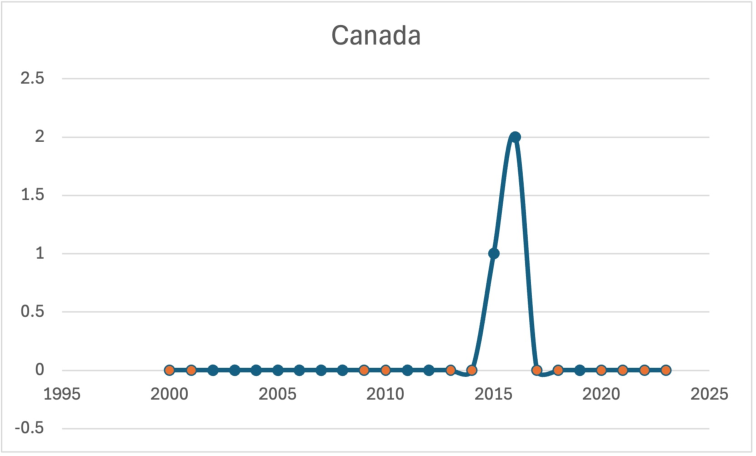
\includegraphics[width=0.45\linewidth]{../rsrc/other_policies/Canada_policy_nearMiss}
            }\\
            \caption{Mitigated Cybercrime Attempts Visualization}\label{fig:mitigated-attempts}
        \end{figure}

    \subsubsection*{Analysis of Cybercrime Reporting Rate} %4.4.2
        In terms of cybercrime reporting rates, the available data for analysis is limited.
        Taking the United States and the United Kingdom as examples, we plot the reporting rate over time in Figure
        ~\ref{fig:reported-attempts}.
        From the graph alone, it appears that
        the \textbf{Presidential Policy Directive 21 (PPD-21) (2013)} in the United States and
        the implementation of \textbf{The General Data Protection Regulation (GDPR) (2018)}
        in the United Kingdom have had a positive impact on increasing reporting rates.
        However, due to the limited amount of data, there is significant noise in the results.
        In reality, the majority of laws and policies do not seem to have a substantial effect on improving reporting rates.
        \begin{figure}[htb]
            \centering
            \subfloat[US\cite{us}]{
                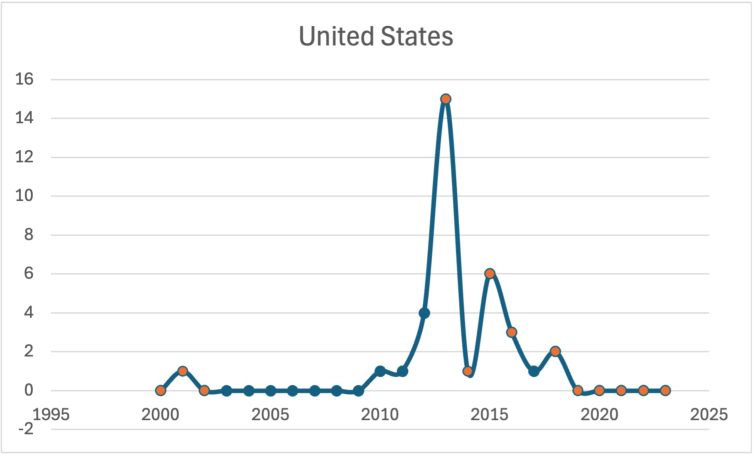
\includegraphics[width=0.45\linewidth]{../rsrc/other_policies/US_policy_suspected}
            }\hfill
            \subfloat[UK\cite{uk}]{
                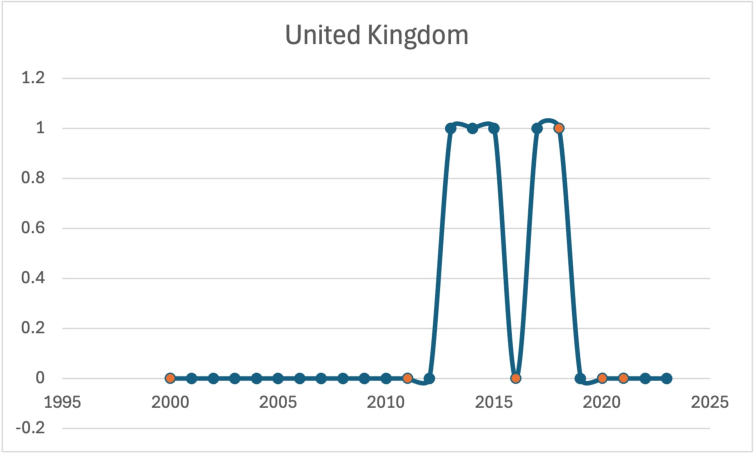
\includegraphics[width=0.45\linewidth]{../rsrc/other_policies/UK_policy_suspected}
            }\\
            \caption{Reported Cybercrime Attempts Visualization}\label{fig:reported-attempts}
        \end{figure}

\subsection{A Poisson Regression Model with Time Leg effect}\label{subsec:a-poisson-regression-model-with-time-leg-effect} %4.5
    From the above data,
    we can intuitively find the benefits of legal policies on cybercrime governance in different countries from 2000 to 2023.
    Based on this, we need to consider the timeliness of the law, that is,
    a certain law may have little benefit for the cybercrime control in the current year,
    but it will be effective for the network control in the next few years.
    Therefore, we do this by using a Poisson regression model and introducing a time lag effect.
    The model is described as:
    \begin{equation}
        \log(\mathbb{E}[Crime_t]) = \beta_0 + \sum_{k=1}^{K} \beta_k Bill_{t-k}\label{eq:4-5-1}
    \end{equation}
    where
    \begin{itemize}
        \item \(\mathbb{E}\) is the expected crime number in the year \(t\),
        \item \(\beta_0\) is the natural logarithm of the baseline crime rate when all explanatory variables are zero,
        \item \(\beta_1, \beta_2, \beta_3\) represent the marginal impact of bills on the crime rate (on a logarithmic scale)
            in the first, second, and third year after passage respectively,
        \item \(Bill_{t-k}\) is the number of bills passed in year \(t-k\) (\(k\) = 1,2,3), and
        \item \(K\) is the greatest lagged number.
    \end{itemize}

    The reason why the linear regression model is not used is that the obtained \(R2\) value is very low,
    indicating that the relationship between the time of bill issuance and the crime rate is not obvious.
    The time lag effect is to get the effect that a bill issued in a given year is likely to have in a lagged number of years.

    Because the Poisson regression analysis also needs to be based on a certain amount of data to ensure the accuracy of the conclusion,
    we choose a few countries that have suffered a large number of cyberattacks for analysis.
    Included: United States, United Kingdom, Canada, Japan, Costa Rica as Figure~\ref{fig:the-poisson-regression} shows.
    \begin{figure}[htb]
        \centering
        \subfloat[United States]{
            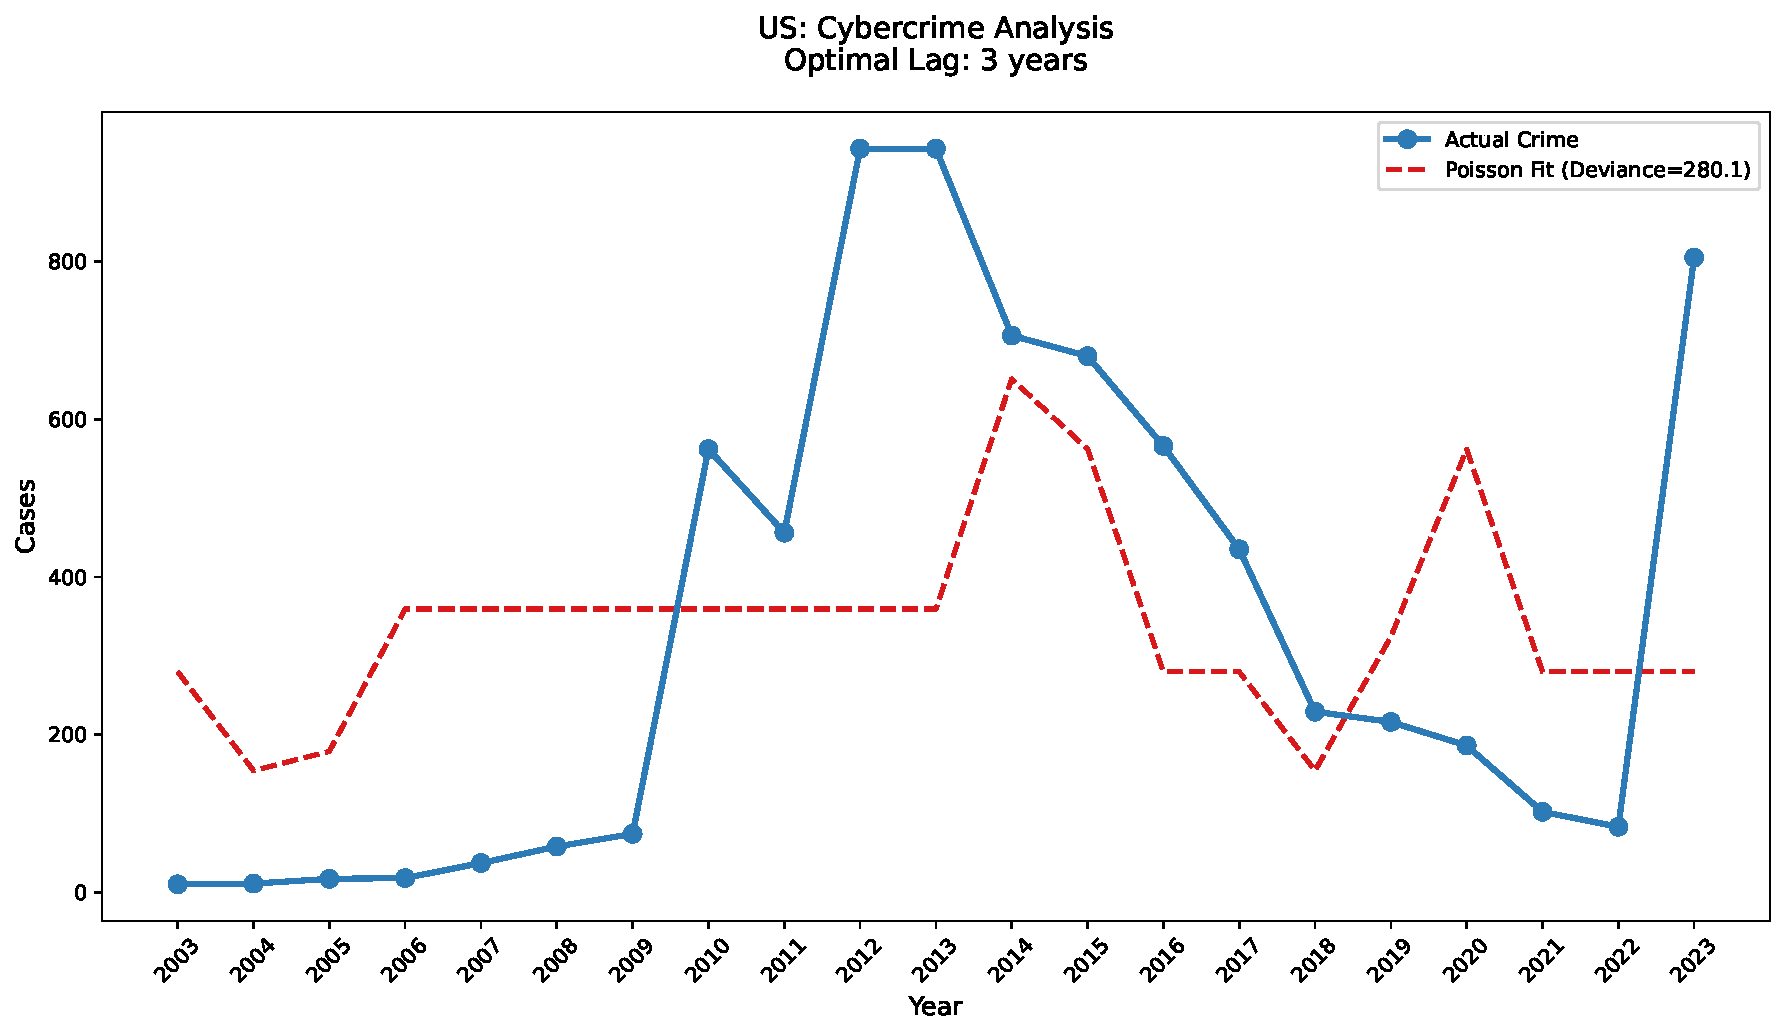
\includegraphics[width=0.45\linewidth]{../rsrc/policy_time/US_Analysis}
        }\hfill
        \subfloat[United Kingdom]{
            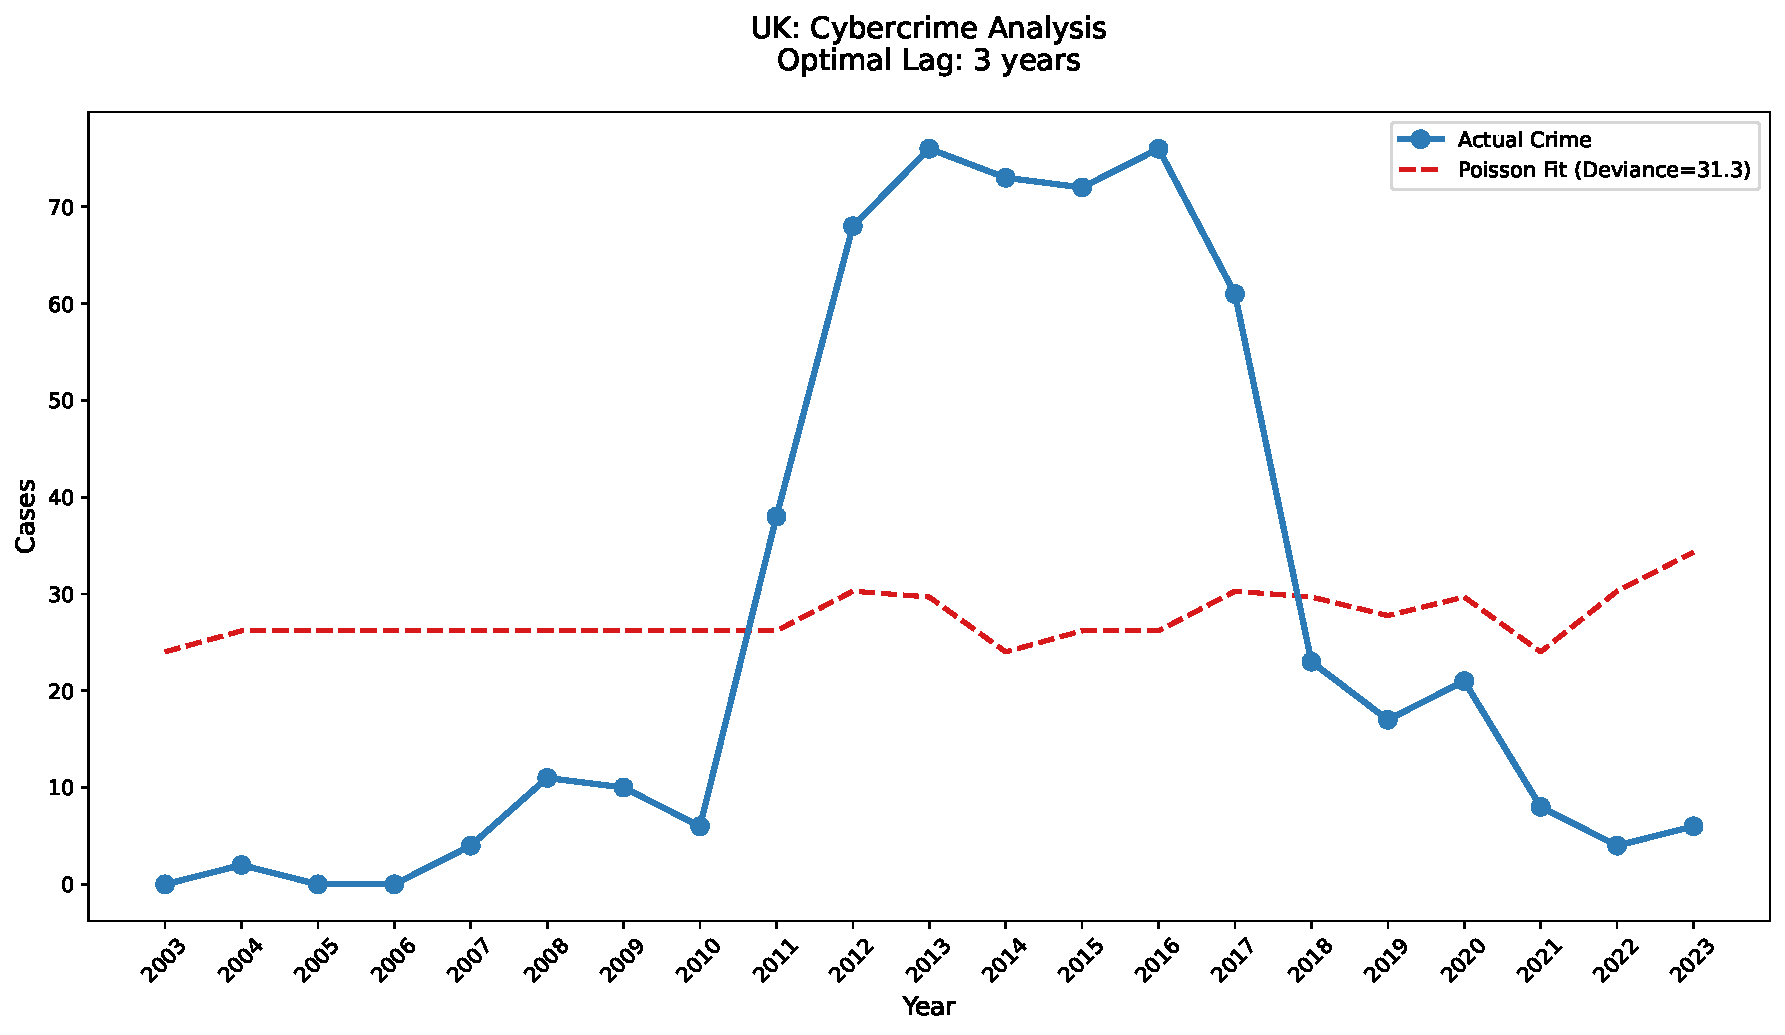
\includegraphics[width=0.45\linewidth]{../rsrc/policy_time/UK_Analysis}
        }\\
        \subfloat[Canada]{
            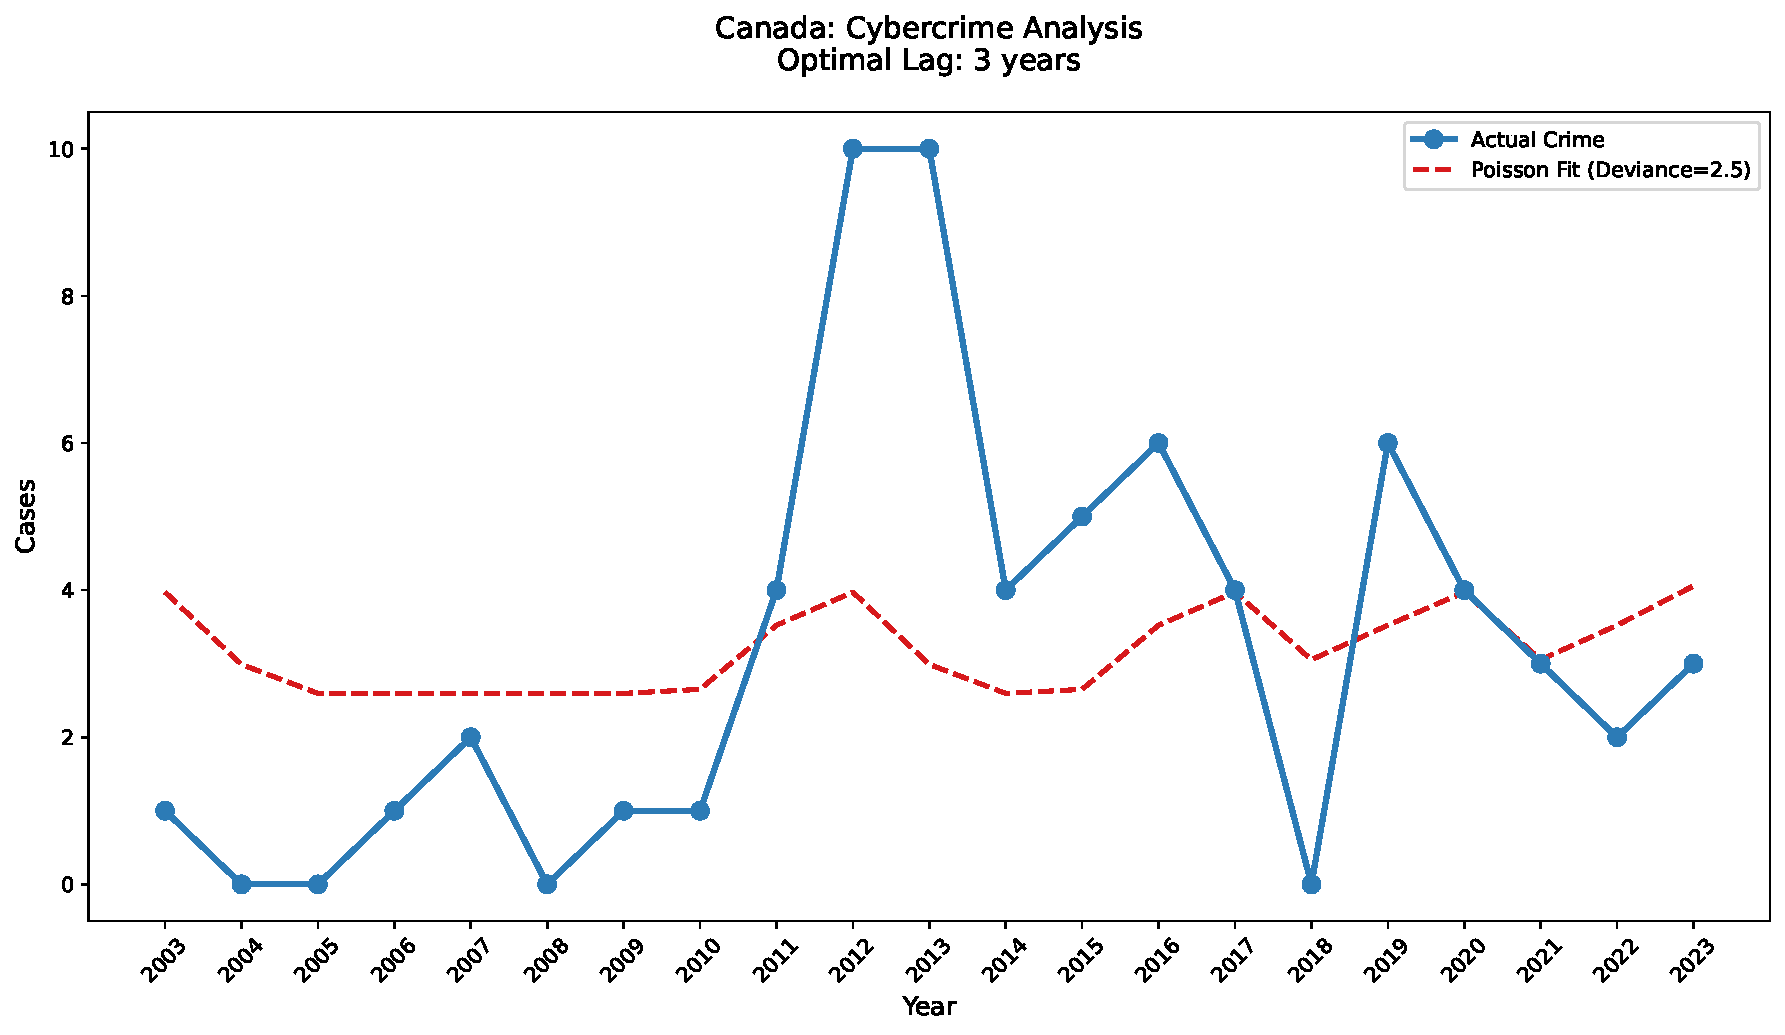
\includegraphics[width=0.3\linewidth]{../rsrc/policy_time/Canada_Analysis}
        }\hfill
        \subfloat[Japan]{
            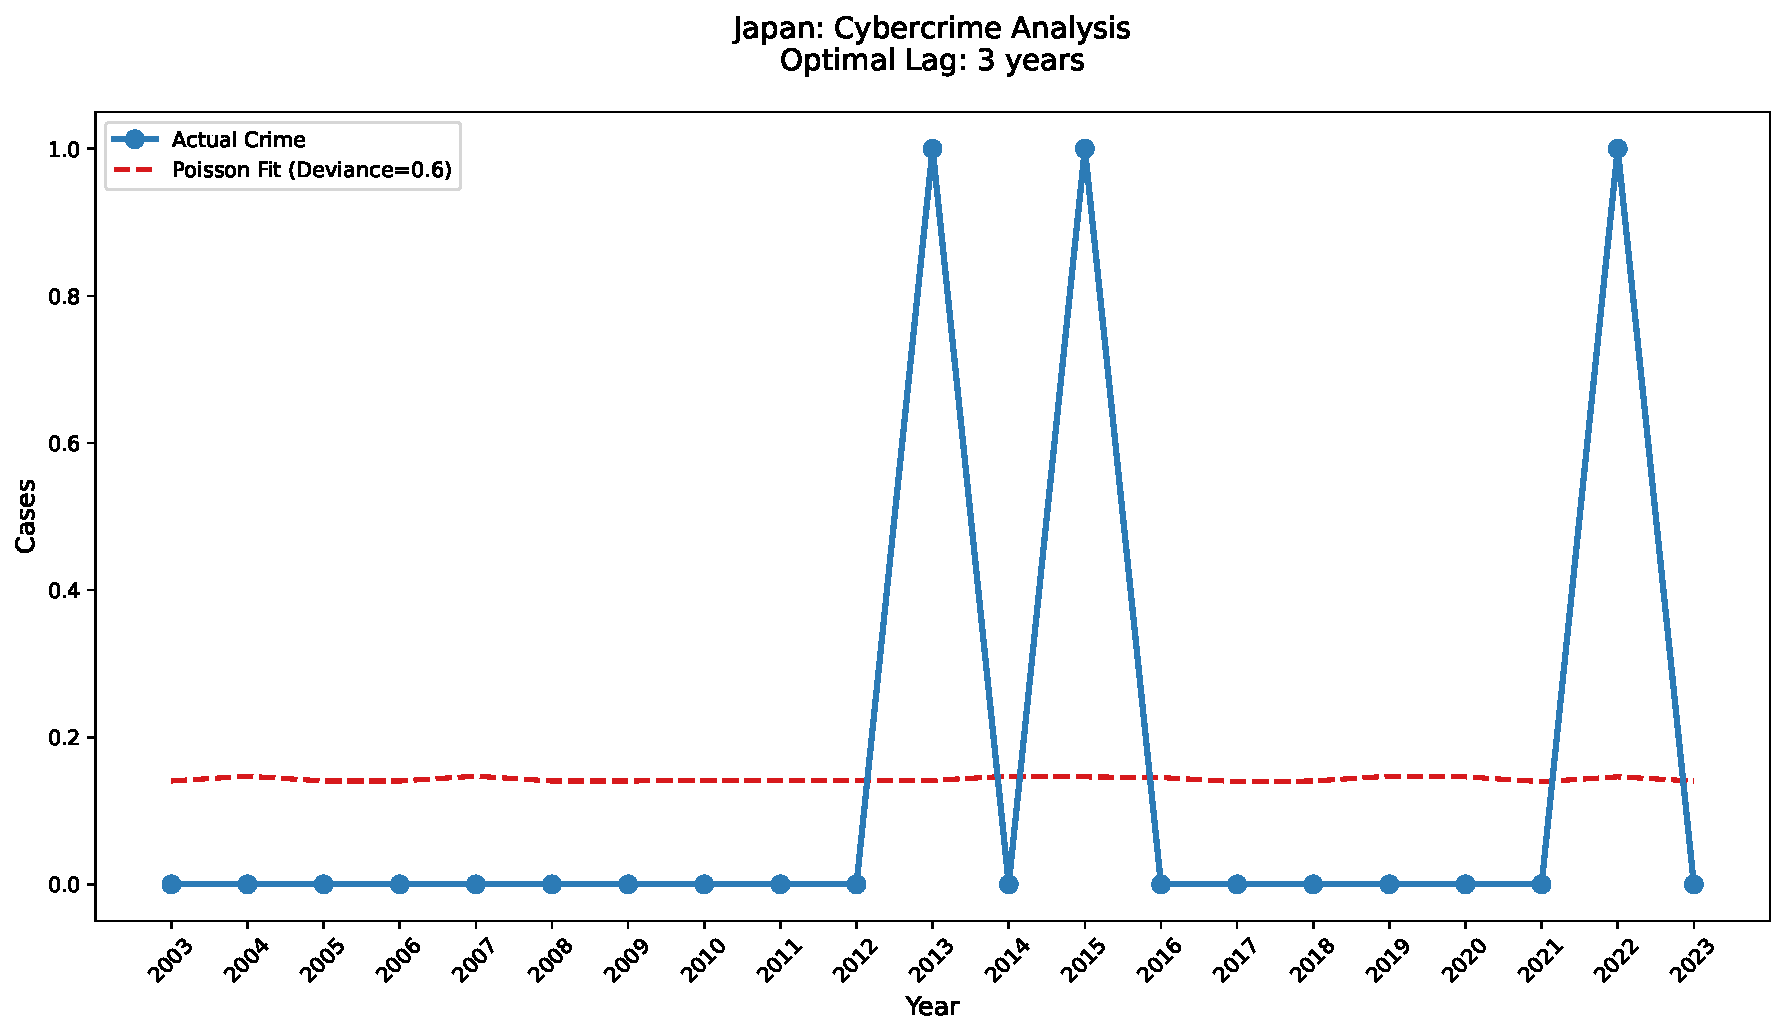
\includegraphics[width=0.3\linewidth]{../rsrc/policy_time/Japan_Analysis}
        }\hfill
        \subfloat[Costa Rica]{
            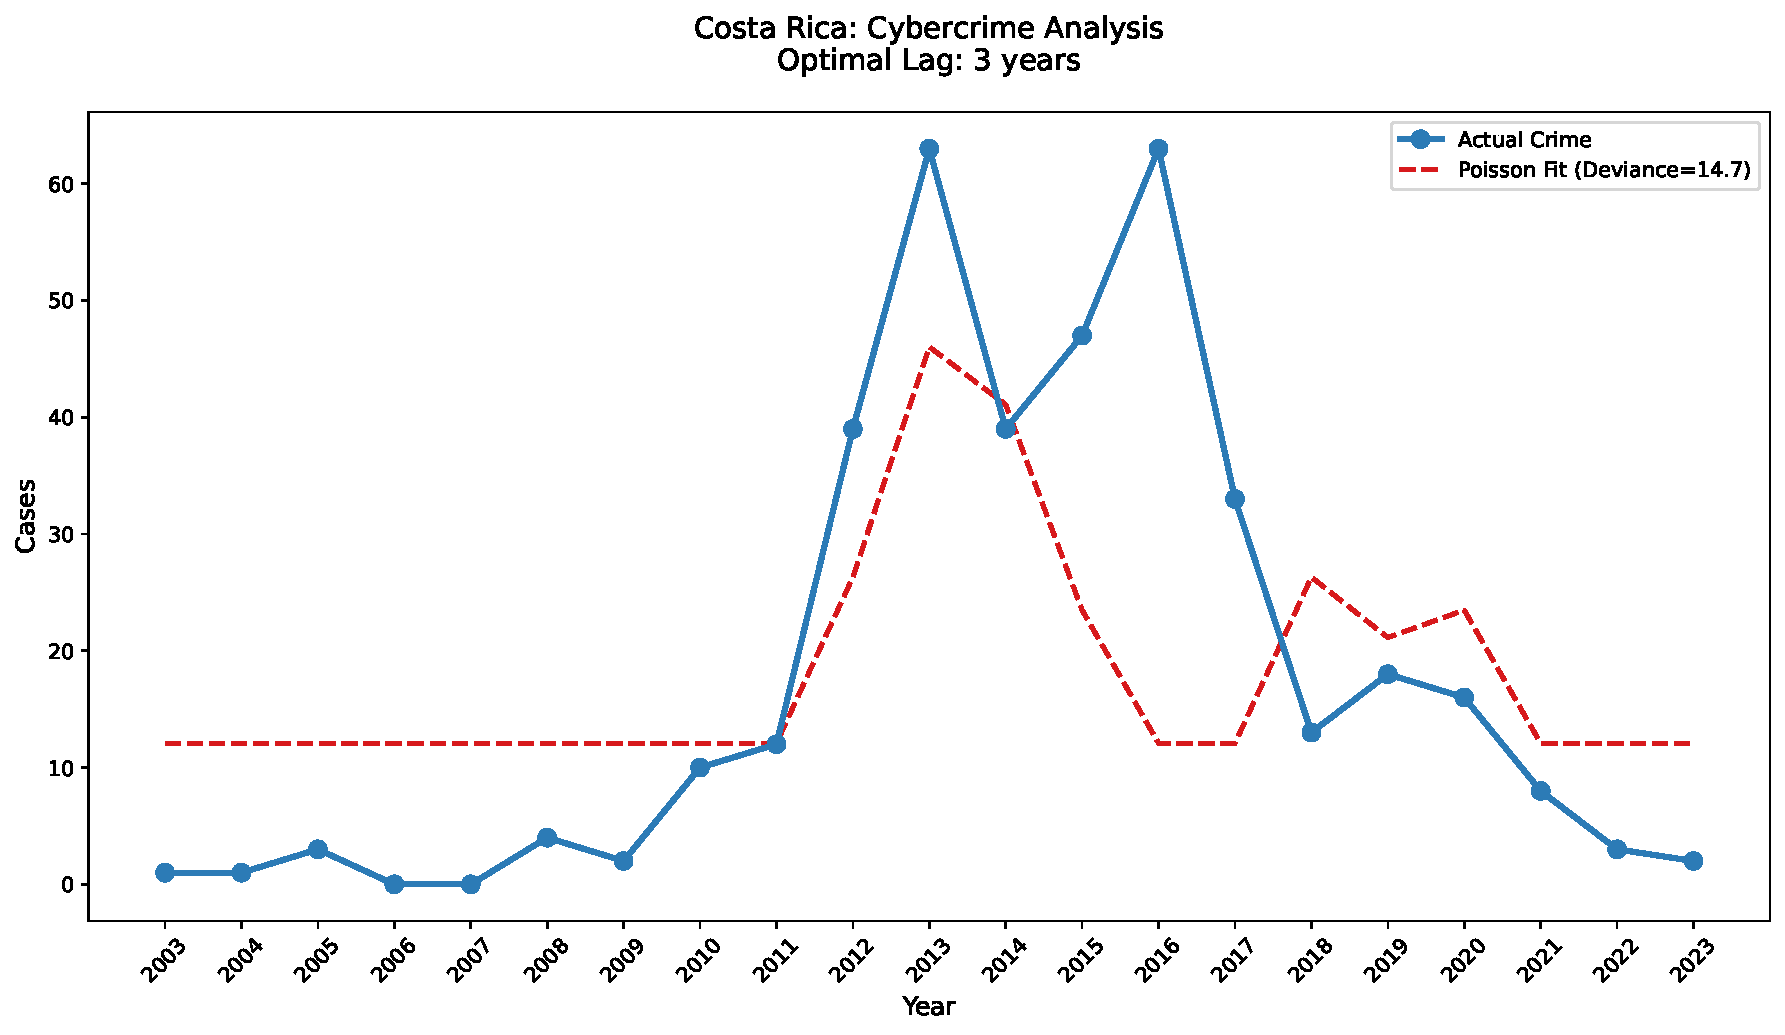
\includegraphics[width=0.3\linewidth]{../rsrc/policy_time/Costa Rica_Analysis}
        }\\
        \caption{Poisson Regression Analysis of Cybercrime Trends}\label{fig:the-poisson-regression}
    \end{figure}

    Based on these, conclusions are as follows:
    \subsubsection*{Canada} % 4.5.1
        The model fits very well,
        indicating that the bill had a significant impact on cybercrime 3 tears after its passage.
        Canada's crime data are less volatile and
        may reflect effective enforcement of its cybersecurity policies or lower crime rates per capita.
        Low bias values indicate a clear relationship between the number of bills and crime rates.
        \begin{itemize}
            \item Best lag period: 3 years.
            \item Poisson bias: 2.5 (very low).
            Actual crime trends: low number of crimes (peak around 10).
        \end{itemize}
    \subsubsection*{Costa Rica} % 4.5.2
        The model is a fair fit, with higher bias than Canada but lower bias than the United States.
        It may indicate that the long-term effects of the Act are present,
        but the data fluctuates greatly or is interfered by other factors
        (e.g., economic conditions, technological developments).
        \begin{itemize}
            \item Best lag period: 3 years.
            \item Poisson bias: 14.7 (medium).
            \item Actual crime trends: moderate number of crimes (peak around 60).
        \end{itemize}
    \subsubsection*{Japan} % 4.5.3
        The bias value is extremely low, but the actual crime number is almost zero,
        possibly reflecting incomplete data recording or indeed rare cybercrime in Japan.
        Although the model fits well, 
        the significance of policy analysis is limited, and the accuracy of data needs to be verified.
        \begin{itemize}
            \item Best lag period: 3 years.
            \item Poisson bias: 0.6 (very low).
            \item Actual crime trends: very low number of crimes (peak around 1).
        \end{itemize}
    \subsubsection*{United Kingdom} % 4.5.4
        UK has a poor model fit, indicating a weak relationship between bills and crime rates.
        \begin{itemize}
            \item Best lag period: 3 years.
            \item Poisson bias: 31.3 (high).
            \item Actual crime trends: Numbers not explicitly shown.
        \end{itemize}
        Possible reasons include:
        \begin{itemize}
            \item Crime data influenced by multiple factors (e.g., transnational cyberattacks).
            \item Delayed or limited implementation of the bill.
        \end{itemize}
    \subsubsection*{United States} % 4.5.5
        US is a very poor fit,
        indicating that the current model does not explain the relationship between bills and crime rates.
        \begin{itemize}
            \item Best lag period: 3 years.
            \item Poisson bias: 280.1 (very high).
            \item Actual crime trends: High number of crimes (e.g.\ 562 in 2010).
        \end{itemize}
        The main reasons may include:
        \begin{itemize}
            \item Outlier impact: spike in 2010.
            \item Data complexity: US cybercrime may involve more dynamic factors
                (e.g., technological advances, scale of hacking).
            \item Policy limitations: Increasing the number of laws alone will not necessarily curb high crime rates.
                A combination of law enforcement and technology is needed.
        \end{itemize}

        Therefore, we can know that the effect of each law on the average of the above countries
        can affect the Internet crime rate in the next 3 years.
        Among them, Canada has the highest revenue from cybercrime governance;
        The results of Japan show that laws and policies are good for the proceeds of cybercrime;
        Due to the limited amount of data,
        Costa Rica can only preliminarily determine that the legal policy has a good effect on its cybercrime control.
        The United Kingdom's laws are less favourable to the proceeds of cybercrime;
        The United States has the worst legal policies for cybercrime.
        In many cases, the release of laws does not directly lead to a decrease in crime rates.
\subsection{Conclusions on the impact of laws and policies on Internet crime rates}
\label{subsec:conclusions-on-the-impact-of-laws-and-policies-on-internet-crime-rates} % 4.6
    From the above information, we can learn that the impact of legal policies on cybercrime has a significant time lag effect,
    that is, the time when legal policies really work may be several years in the future.
    Moreover, the effects of laws and policies vary from country to country.
    For T1 countries like the United States with a large population,
    the increase in the number of laws may not directly reduce the crime rate.
    Even if the laws are issued frequently, it is difficult to curb the growth of the number of cyber crimes,
    indicating that there may be some problems in the content or implementation of the laws.
    But for countries such as Canada, the number of laws is consistent but the effect is significant,
    which indicates that the laws are well-designed and effectively implemented.
    Outliers in the data, such as the spike in cybercrime in the US in 2010, can skew the true trend to some extent.
    Finally, long-term policy effects are better than short-term ones.
    Therefore, it is necessary to comprehensively consider the above factors to control the Internet crime rate.
